\documentclass[10pt]{article}
\usepackage{common/acl-ijcnlp2009}
\usepackage{times}
\usepackage{latexsym}
\usepackage{common/prettyref}
\usepackage{common/jeffe}
\usepackage{common/hyphen}
\usepackage{latexsym}
\usepackage{subfigure}
\usepackage{graphicx}
\usepackage[applemac]{inputenc}

\newrefformat{tab}{Table \ref{#1}} 
\newrefformat{fig}{Figure \ref{#1}} 
\newrefformat{eqn}{(\ref{#1})} 
\newcommand{\ignore}[1]{}


\newcommand{\nt}[2]{\textrm{#1}_{\framebox[5pt]{\scriptsize #2}}}
\newcommand\bleu{\textsc{Bleu}}
\newcommand\giza{{GIZA++}}
\newcommand\boe{\mathbf{e}}
\newcommand\bof{\mathbf{f}}
\newcommand{\ind}[1]{{\fboxsep1pt\raisebox{-.5ex}{\fbox{{\tiny #1}}}}}
% allows margin notes
%\newcommand\margin[1]{} % hide them!!!
\newcommand\margin[1]{\mbox{}\marginpar{\raggedright\hspace{0pt}\tiny\em#1}}
\addtolength{\marginparwidth}{-3ex}

\newcommand{\ts}{\ensuremath{\vec{t}}}
\newcommand{\es}{\ensuremath{\vec{e}}}
\newcommand{\rs}{\ensuremath{\vec{r}}}
\newcommand{\condon}{\hspace{0pt} | \hspace{1pt}}
\newcommand{\but}[2]{\ensuremath{{\bf #1}_{-#2}}}
\newcommand{\blt}[2]{\ensuremath{{\bf #1}_{<#2}}}
\newcommand{\pu}{\ensuremath{P_0}}
\renewcommand{\vec}[1]{{\bf #1}}
\newcommand{\emin}{\ensuremath{\es^-}}

\newcommand{\bibsnip}{\vspace{-1ex}}

%% sloppy linebreaks
%\sloppy

%% no extra spacing after dots
%\frenchspacing

\makeatletter
\setlength{\columnsep}{3mm} % this one's nasty!!!

%\setlength{\topmargin}{0in}
%\setlength{\headheight}{0in}
%\setlength{\headsep}{-0.2in}
%\setlength{\textheight}{10.0in}
%\setlength{\oddsidemargin}{0in}
%\setlength{\textwidth}{6.5in}
\setlength\titlebox{1.65in}
\renewcommand{\baselinestretch}{0.96}
\setlength{\textfloatsep}{3mm}
\setlength{\floatsep}{1.5mm}


\title{Unsupervised models of Synchronous Grammar Induction for SMT}
\author{
  Phil Blunsom\\ 
  %\vspace{6pt} 
  Phil.Blunsom@comlab.ox.ac.uk\\
%  {\rm $^*$Computing Laboratory}\\
  University of Oxford\\
 \And
  Alex Clark\\
  %\vspace{6pt} 
  alexc@cs.rhul.ac.uk\\
%  {\rm $^\textrm{\textdagger}$Department of Computer Science}\\
  Royal Holloway University
 \And
  Trevor Cohn\\
  %\vspace{6pt} 
  T.Cohn@dcs.shef.ac.uk\\
%  {\rm $^\textrm{\textdagger}$Department of Computer Science}\\
  University of Shefield
\\
 \AND
  Chris Dyer\\
  %\vspace{6pt} 
  redpony@umd.edu\\
%  {\rm $^\textrm{\textdagger}$Department of Computer Science}\\
  University of Maryland
 \And
  Adam Lopez\\
  %\vspace{6pt} 
  alopez@inf.ed.ac.uk\\
%  {\rm $^\textrm{\textdagger}$Department of Computer Science}\\
  University of Edinburgh 
}

\begin{document}
\maketitle

\begin{abstract}
Synchronous grammar transducers have made a big impact in the field of machine translation in recent years. 
However, current techniques for acquiring translation grammars are either overly simplistic or else too heavily reliant on the availability of high-quality statistical parsers.
We propose the development of algorithms for large-scale unsupervised synchronous grammar induction. 
Using advanced clustering techniques from machine learning we aim to induce grammars which use a rich set of non-terminals, %, in contrast to many existing approaches which have only one.
thereby producing high quality translation models for language pairs solely using a parallel corpus. %, without relying on treebank parsers.
\end{abstract}

%%Research into statistical machine translation has changed dramatically in recent years with the introduction of grammar-based transducers (e.g., Chang's Hiero and USC/ISI's syntax-based system). 
%A critical component of synchronous grammar translation models is their \emph{grammar} which encodes translational equivalence and licenses reordering between tokens in the source and target languages. 
%There is considerable scope for improving beyond current techniques for automatically acquiring synchronous grammars from bilingual corpora, which seek to find either extremely simple grammars with only one non-terminal or else rely on treebank-trained parsers.
%The simple grammars are incapable of representing constituency information, while the richer grammars limit the systems' portability to new target languages while enforcing a restrictive notion of linguistic constituency. 
%Instead we propose to develop an unsupervised method for large-scale unsupervised synchronous grammar induction using multiple non-terminal symbols to represent contextual information.
%In such a way we can harness the benefits of a richer grammar without the limiting data requirements or linguistic constraints.

The last decade of research in Statistical Machine Translation (SMT) has seen rapid progress. %with small scale research systems maturing into large commercial products and ubiquitous online tools. %\footnote{e.g., translate.google.com, www.systran.co.uk, www.languageweaver.com} 
Unfortunately the success of SMT has not been uniform; 
%current state-of-the-art translation output varies markedly in quality depending on the languages being translated. 
%Those language pairs that are 
closely related language pairs 
%(e.g., English and French) 
can be translated with a high degree of precision, while for distant pairs 
%(e.g., English and Chinese) 
the result is far from acceptable. 
It is tempting to argue that SMT's current limitations can be overcome simply by increasing the amount of data on which the systems are trained. 
However, large scale evaluation campaigns for Chinese~$\rightarrow$~English translation have not yielded the expected gains despite the increasing size of the models. 
%While many researchers are tackling these issues, their proposed solutions are limited by focusing on more expressive models of translation rather than addressing the issue of how, and what, translation units are learnt a priori.

Those models which have been most successful for translating between structurally divergent language pairs have been based on synchronous tree substitution grammars (STSG). 
%However these successes have been tempered by a reliance on high quality monolingual parse trees on the output side of the translation model, severely restricting the applicability of such models to the case of translating into English.
A critical component of these translation models is their \emph{grammar} which encodes translational equivalence and licenses reordering between tokens in the source and target languages. 
There is considerable scope for improving beyond current techniques for automatically acquiring synchronous grammars from bilingual corpora, which seek to find either extremely simple grammars with only one non-terminal or else rely on treebank-trained parsers.
The simple grammars are incapable of representing the substitutability of a constituent, while the richer grammars limit the systems' portability to new target languages while enforcing a restrictive notion of linguistic constituency (Figure \ref{fig:models}). 
%A further, but more subtle, limitation of these models is the assumption that the particular brand of linguistic structure assigned by a parser (usually a form of phrase structure grammar learnt from the Penn. Treebank) is predominantly isomorphic to that of the input language; an assumption which is rarely true for distantly related language pairs (or even closely related ones: Figure \ref{fig:models}).

Clearly there is a need for research into the unsupervised induction of synchronous grammar based translation models.
Previous research has focussed on structured learning approaches requiring costly global inference over translation pair derivations, limiting the ability of these models to be scaled to large datasets.
Here we propose the more pragmatic approach of embracing existing algorithms for inducing unlabelled SCFGs (e.g. the popular Hiero model) as a starting point, and then using state-of-the-art clustering and topic modelling algorithms to independently learn syntactic congruence classes for translation rules in the grammar.

\begin{figure}
  \subfigure[Formal syntax]{\includegraphics[scale=0.34]{JeNeVeuxPasTravailler-hiero.pdf}}
  \subfigure[Linguistic syntax]{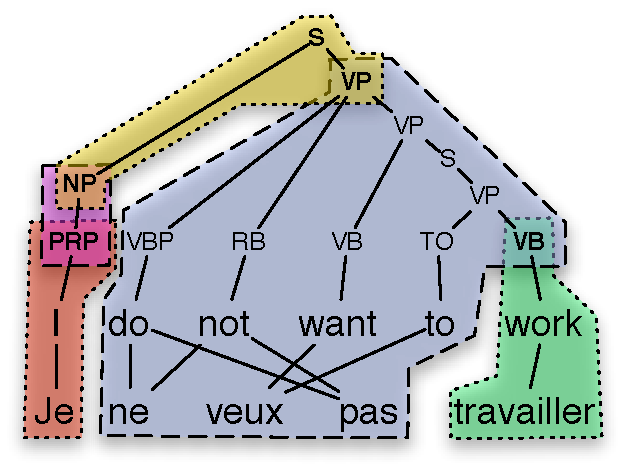
\includegraphics[scale=0.34]{JeNeVeuxPasTravailler-tsg.pdf}}
\caption{What is the best syntactic structure for SMT?}
\label{fig:models}
\end{figure}

The agenda of the workshop will be motivated by two goals: (1) to investigate the role of constituency and syntactic congruence in synchronous grammars; (2) to develop scalable algorithms for assigning labels to translation rules in Hiero style grammars. These algorithms will be implemented within the Joshua decoder.

\paragraph{1) Synchronous constituency} 
The first goal deals with the question of the degree to which practical synchronous grammar SMT systems should be based on linguistic or non-linguistic models of syntax.
Previous work has assumed a linguistic motivation, but there is a compelling argument that a more appropriate representation may be one which specifically addresses the divergence between a given language pair (Figure~\ref{fig:models}).
Such a grammar might simply encode the number of tokens in the constituent being generated, the number of reordering operations on the path from the root to that constituent, or whether a constituent prefers to reorder in a specific direction.

\paragraph{2) Clustering translation units} 
The second goal will be to adapt existing unsupervised clustering techniques, such as Latent Dirichlet Allocation (LDA) and Hierarchical Dirichlet Processes (HDPs), to the task of assigning equivalence classes to phrase translations.
Inspired by work in monolingual PCFG learning, we will investigate generative models which describe the production of phrase translations in terms of sequences of tokens (or word classes) and their observed contexts.

By investigating these goals in the context of a CLSP workshop we hope to both generate interest and further research into widely applicable unsupervised techniques for synchronous grammar induction, and to provide a benchmark implementation ready for wide adoption within the SMT research community.
\end{document}
